\documentclass[11pt]{article}

\usepackage[a4paper,margin=1in]{geometry}
\usepackage{amsmath,amssymb,amsthm}
\usepackage{booktabs}
\usepackage{graphicx}
\usepackage{natbib}
\usepackage{url}
\usepackage{placeins}

\newtheorem{lemma}{Lemma}
\newtheorem{proposition}{Proposition}
\newtheorem{theorem}{Theorem}

\newcommand{\Sone}{\mathbb S^1}
\newcommand{\Td}{\mathbb T^d}
\newcommand{\R}{\mathbb R}
\newcommand{\E}{\mathbb E}
\newcommand{\HSIC}{\operatorname{HSIC}}
\newcommand{\MMD}{\operatorname{MMD}}
\newcommand{\tr}{\operatorname{tr}}

\title{Geometry-aware HSIC independence testing for circular, toroidal and circular-linear data}
\author{}
\date{}

\begin{document}
\maketitle

\begin{abstract}
The Hilbert--Schmidt independence criterion is a classical kernel measure of statistical dependence, but its practical use with directional variables requires kernels that respect the sample space.  This paper gives a compact formulation of HSIC independence testing for circular, toroidal and circular-linear data.  For circular variables, the construction uses the von Mises kernel \(k_\kappa(\theta,\theta')=\exp\{\kappa\cos(\theta-\theta')\}\), \(\kappa>0\), and provides a self-contained Fourier proof that this kernel is characteristic on \(\mathbb S^1\).  Product Fourier expansions give characteristic kernels on finite tori, while pairing the circular kernel with a Gaussian kernel gives a practical circular-linear test under standard product-kernel assumptions.  The empirical procedure uses the biased Gram-matrix HSIC statistic with add-one permutation calibration.  We also describe a standardized multi-scale version that searches over concentration parameters and includes this search in the permutation calibration.  Reproducible R scripts are provided for null calibration checks, power studies, sensitivity analyses and an applied Noshiro directional-data example.  The aim is not to introduce HSIC, characteristic kernels, or circular independence tests as new.  Rather, the paper supplies a statistically explicit and computationally reproducible workflow for applying HSIC while preserving periodic geometry.
\end{abstract}

\noindent\textbf{Keywords:} circular data; characteristic kernels; Hilbert--Schmidt independence criterion; kernel mean embedding; permutation test; torus; von Mises kernel.

\section{Introduction}

Directional data arise when observations live on circles, tori or products involving directional and Euclidean components.  Examples include wind direction and temperature, movement direction and speed, paired angular measurements, and toroidal coordinates such as dihedral angles.  In these settings, independence testing should respect periodicity and product geometry.  Applying Euclidean kernels directly to raw angular coordinates can create boundary artifacts at \(0\) and \(2\pi\), and can obscure rotation-invariant structure.

This paper focuses on the circle \(\Sone\), finite tori \(\Td=(\Sone)^d\), and mixed spaces \(\Sone\times\R^p\).  The method is based on HSIC \citep{gretton2005hsic,gretton2008kernel}, kernel mean embeddings and characteristic kernels \citep{sriperumbudur2010hilbert,sriperumbudur2011universality}.  Circular and directional statistics are well established \citep{mardia1975directional,mardiajupp2000directional,fisher1993circular,ley2017modern,pewsey2021recent}, as are circular independence tests and diagnostics \citep{jammalamadaka2001topics,shieh1994weighted,garciaportugues2024trigonometric}.  The point of this paper is therefore not to present HSIC or circular independence testing as new.  It is to give a mathematically explicit and reproducible specialization of HSIC to common directional sample spaces.  The useful addition is the combination of geometry-aware kernels, characteristicness arguments and permutation-calibrated implementation in a single workflow for circular, toroidal and circular-linear data.

The resulting specialization has three linked components.  First, it uses the von Mises kernel to build HSIC tests for circular-circular variables and gives a self-contained Fourier proof that this kernel is characteristic on \(\Sone\).  Second, it extends the same argument to finite tori through product kernels and multi-index Fourier expansions, and it treats circular-linear data by pairing the circular kernel with a Gaussian kernel on \(\R^p\).  Third, it turns these population constructions into a reproducible empirical procedure based on the biased Gram-matrix HSIC statistic, permutation calibration under exchangeability and a standardized multi-scale tuning strategy in which the search over concentration parameters is included in the calibration.  The accompanying R code implements the tests, simulation studies, sensitivity checks and Noshiro data analysis used below.

The scope is intentionally limited.  Spherical and hyperspherical variables are not treated as a main contribution in this version.  They are discussed only as future work requiring a separate harmonic-analysis proof.

\section{Background: HSIC and characteristic kernels}

Let \(\mathcal X\) be a topological space with Borel \(\sigma\)-field \(\mathcal B(\mathcal X)\), and let \(k:\mathcal X\times\mathcal X\to\mathbb R\) be a bounded measurable positive definite kernel with reproducing kernel Hilbert space \(\mathcal H_k\).  For a Borel probability measure \(P\), the kernel mean embedding is the Bochner integral
\[
  \mu_P=\int k(x,\cdot)\,dP(x).
\]
For Borel probability measures \(P\) and \(Q\), the maximum mean discrepancy is
\[
  \MMD_k(P,Q)=\|\mu_P-\mu_Q\|_{\mathcal H_k}.
\]
The kernel is characteristic to Borel probability measures when \(\MMD_k(P,Q)=0\) implies \(P=Q\).  Equivalently, the mean embedding is injective on the class of Borel probability measures under consideration \citep{sriperumbudur2010hilbert,sriperumbudur2011universality}.

For random elements \(X\in\mathcal X\) and \(Y\in\mathcal Y\), with Borel laws \(P_{XY}\), \(P_X\) and \(P_Y\), HSIC can be written as the squared MMD between the joint law and the product of the marginal laws:
\[
  \HSIC_{k,\ell}(X,Y)
  =
  \MMD^2_{k\otimes \ell}\{P_{XY},P_X\otimes P_Y\}.
\]
If the product kernel \(k\otimes\ell\) is characteristic on \(\mathcal X\times\mathcal Y\), then \(\HSIC_{k,\ell}(X,Y)=0\) if and only if \(P_{XY}=P_X\otimes P_Y\), that is, \(X\) and \(Y\) are independent \citep{gretton2005hsic,gretton2008kernel}.  This population identity is the target calibrated empirically below.

\section{Von Mises kernels on the circle}

We identify \(\Sone\) with \(\mathbb R/(2\pi\mathbb Z)\), equipped with its Borel \(\sigma\)-field.  For \(\kappa>0\), define
\[
  k_\kappa(\theta,\theta')=\exp\{\kappa\cos(\theta-\theta')\}.
\]
The kernel is continuous, bounded, \(2\pi\)-periodic in each argument and rotation invariant.  Its Fourier expansion is
\[
  \exp\{\kappa\cos t\}
  =
  \sum_{m\in\mathbb Z} I_m(\kappa)e^{imt},
\]
where \(I_m\) is the modified Bessel function of the first kind \citep{abramowitz1964handbook}.  For \(\kappa>0\), \(I_m(\kappa)>0\) for every \(m\in\mathbb Z\).  The series converges absolutely and uniformly because the coefficients are nonnegative and
\[
  \sum_{m\in\mathbb Z} I_m(\kappa)=\exp(\kappa)<\infty .
\]
The strict positivity of every coefficient is the key point: no Fourier frequency is suppressed by the kernel.

\begin{lemma}[Positive definiteness]
For every \(\kappa>0\), \(k_\kappa\) is positive definite on \(\Sone\).
\end{lemma}

\begin{proof}
Let \(c_1,\ldots,c_n\in\mathbb C\) and \(\theta_1,\ldots,\theta_n\in\Sone\).  By absolute uniform convergence of the Fourier series,
\[
  \sum_{i,j} c_i\overline{c_j}k_\kappa(\theta_i,\theta_j)
  =
  \sum_{m\in\mathbb Z} I_m(\kappa)
  \left|\sum_i c_i e^{im\theta_i}\right|^2
  \ge 0.
\]
Thus every Gram matrix generated by \(k_\kappa\) is Hermitian nonnegative definite.  Since the kernel is real-valued and symmetric, this is the usual positive definiteness condition.
\end{proof}

\begin{theorem}[Characteristicness on the circle]
For every \(\kappa>0\), the von Mises kernel \(k_\kappa\) is characteristic on \(\Sone\).
\end{theorem}

\begin{proof}
Let \(P\) and \(Q\) be Borel probability measures on \(\Sone\), and let \(\nu=P-Q\), a finite signed Borel measure.  Define its Fourier coefficients by
\[
  \widehat\nu_m=\int_{\Sone} e^{im\theta}\,d\nu(\theta),
  \qquad m\in\mathbb Z.
\]
Using the Fourier expansion and Fubini's theorem, justified by boundedness of \(k_\kappa\) and absolute uniform convergence,
\[
\MMD^2_{k_\kappa}(P,Q)
=
\iint k_\kappa(\theta,\theta')\,d\nu(\theta)d\nu(\theta')
=
\sum_{m\in\mathbb Z} I_m(\kappa)|\widehat\nu_m|^2.
\]
If this quantity is zero, strict positivity of \(I_m(\kappa)\) for every \(m\) implies \(\widehat\nu_m=0\) for all \(m\in\mathbb Z\).  Finite Borel measures on compact Abelian groups, in particular on \(\Sone\), are uniquely determined by their Fourier coefficients \citep{rudin1962fourier,fukumizu2009groups}.  Hence \(\nu=0\), so \(P=Q\).  Therefore the mean embedding is injective on Borel probability measures, and \(k_\kappa\) is characteristic.
\end{proof}

\section{Toroidal product kernels}

Let \(\Td=(\Sone)^d\), equipped with its Borel \(\sigma\)-field and group operation given by componentwise addition modulo \(2\pi\).  For \(x=(\theta_1,\ldots,\theta_d)\) and \(x'=(\theta'_1,\ldots,\theta'_d)\) in \(\Td\), define the product von Mises kernel
\[
  K_{\boldsymbol\kappa}(x,x')
  =
  \prod_{r=1}^d \exp\{\kappa_r\cos(\theta_r-\theta'_r)\},
  \qquad \kappa_r>0.
\]
Equivalently,
\[
  K_{\boldsymbol\kappa}(x,x')
  =
  \exp\left\{\sum_{r=1}^d\kappa_r\cos(\theta_r-\theta'_r)\right\}.
\]
Writing \(u=x-x'\), the multi-index Fourier expansion is
\[
  K_{\boldsymbol\kappa}(x,x')
  =
  \sum_{m\in\mathbb Z^d}
  a_m(\boldsymbol\kappa)e^{i m^\top (x-x')},
  \qquad
  a_m(\boldsymbol\kappa)=\prod_{r=1}^d I_{m_r}(\kappa_r).
\]
The coefficients satisfy \(a_m(\boldsymbol\kappa)>0\) for every \(m\in\mathbb Z^d\) when all \(\kappa_r>0\), and the expansion converges absolutely and uniformly since
\[
  \sum_{m\in\mathbb Z^d} a_m(\boldsymbol\kappa)
  =
  \prod_{r=1}^d \exp(\kappa_r)<\infty .
\]

\begin{proposition}[Characteristic toroidal product kernel]
If all \(\kappa_r>0\), then \(K_{\boldsymbol\kappa}\) is characteristic on \(\Td\).
\end{proposition}

\begin{proof}
Let \(P\) and \(Q\) be Borel probability measures on \(\Td\), and let \(\nu=P-Q\) be the corresponding finite signed Borel measure.  For \(m\in\mathbb Z^d\), write
\[
  \widehat\nu_m=\int_{\Td} e^{i m^\top x}\,d\nu(x).
\]
As in the one-dimensional case,
\[
  \MMD^2_{K_{\boldsymbol\kappa}}(P,Q)
  =
  \sum_{m\in\mathbb Z^d} a_m(\boldsymbol\kappa)|\widehat\nu_m|^2 .
\]
All coefficients \(a_m(\boldsymbol\kappa)\) are strictly positive, so zero MMD implies \(\widehat\nu_m=0\) for every \(m\in\mathbb Z^d\).  By uniqueness of finite Borel measures from Fourier coefficients on compact Abelian groups \citep{rudin1962fourier}, \(\nu=0\).  Hence \(P=Q\), and the product kernel is characteristic.  The assumption \(\kappa_r>0\) in every coordinate is essential: if one concentration is zero, the kernel is constant in that coordinate and cannot distinguish probability measures that differ only through that marginal direction.
\end{proof}

Consequently, if \(X\in\mathbb T^{d_X}\) and \(Y\in\mathbb T^{d_Y}\) are equipped with product von Mises kernels whose concentration components are all strictly positive, then the joint kernel \(K_X\otimes K_Y\) is itself a product von Mises kernel on \(\mathbb T^{d_X+d_Y}\).  It is therefore characteristic, and population HSIC is zero if and only if \(X\) and \(Y\) are independent.  The circular-circular case is obtained with \(d_X=d_Y=1\).

\section{Circular-linear independence}

Let \(\Theta\in\Sone\) and \(X\in\R^p\).  Use the von Mises kernel \(k_\kappa\) on \(\Sone\) and a bounded characteristic Euclidean kernel \(g\) on \(\R^p\).  The main practical choice is the Gaussian kernel
\[
  g_\sigma(x,x')=\exp\{-\|x-x'\|^2/(2\sigma^2)\},
  \qquad \sigma>0.
\]
The following proposition covers the practical circular-linear kernel used in the implementation.

\begin{proposition}[von Mises times Gaussian kernel]
Let \(\kappa>0\) and \(\sigma>0\).  The product kernel
\[
  K\{(\theta,x),(\theta',x')\}
  =
  k_\kappa(\theta,\theta')g_\sigma(x,x')
\]
is characteristic on \(\Sone\times\R^p\).
\end{proposition}

\begin{proof}
View \(\Sone\times\R^p\) as a locally compact Abelian group, with dual variables \((m,\omega)\in\mathbb Z\times\R^p\).  The von Mises factor has Fourier coefficients \(I_m(\kappa)>0\) for every \(m\in\mathbb Z\).  The Gaussian factor is translation invariant on \(\R^p\) and has a spectral density that is strictly positive for every \(\omega\in\R^p\).  Hence the product spectral measure has support equal to the full dual group \(\mathbb Z\times\R^p\).  By the Fourier characterization of characteristic translation-invariant kernels on locally compact Abelian groups \citep{berg1984harmonic,fukumizu2009groups,sriperumbudur2010hilbert,sriperumbudur2011universality}, the product kernel is characteristic.
\end{proof}

Consequently, for the von Mises times Gaussian kernel, the population identity is
\[
  \HSIC_{k_\kappa,g}(\Theta,X)=0
  \quad\Longleftrightarrow\quad
  \Theta\perp X.
\]
This is the circular-linear testing principle used in the simulations.  It is not presented as a new general theory for arbitrary products of compact and non-compact spaces.  The contribution is the explicit geometry-aware construction using a circular characteristic kernel paired with a standard characteristic Euclidean kernel.  Related directional-linear kernel density and independence methods are developed by \citet{garciaportugues2013kde,garciaportugues2014directionallinear}.  Applications include direction-speed, wind-temperature and movement-covariate studies.

\section{Empirical test and permutation calibration}

Let \((X_i,Y_i)_{i=1}^n\) be paired observations.  For kernels \(k\) and \(\ell\), define the Gram matrices \(K_{ij}=k(X_i,X_j)\) and \(L_{ij}=\ell(Y_i,Y_j)\), and let
\[
  H=I_n-\frac{1}{n}\mathbf 1\mathbf 1^\top.
\]
The biased empirical HSIC statistic is
\[
  \widehat{\HSIC}_n=\frac{1}{n^2}\tr(KHLH).
\]
Equivalently, \(\widehat{\HSIC}_n=n^{-2}\tr(\widetilde K\widetilde L)\), where \(\widetilde K=HKH\) and \(\widetilde L=HLH\).  An unbiased U-statistic version exists, but the biased statistic is stable, nonnegative and simple to compute.  Under permutation calibration, the same statistic is applied to the observed pairing and to every permuted pairing.  Therefore the finite-sample bias of the statistic is not interpreted as an estimator bias correction; it is part of the test statistic whose null distribution is calibrated by permutations.

\begin{center}
\fbox{\begin{minipage}{0.94\textwidth}
\textbf{Algorithm 1. Single-scale permutation HSIC test}
\begin{enumerate}
  \item Choose kernels \(k\) and \(\ell\), including their parameters.
  \item Compute \(K\), \(L\), \(H\), \(\widetilde K=HKH\) and \(\widetilde L=HLH\).
  \item Compute \(T_{\mathrm{obs}}=n^{-2}\tr(\widetilde K\widetilde L)\).
  \item For \(b=1,\ldots,B\), draw a random permutation \(\pi_b\) of \(\{1,\ldots,n\}\), set \(L^{(b)}=P_bLP_b^\top\), where \(P_b\) is the corresponding permutation matrix, and compute
  \[
    T_b=n^{-2}\tr\{KHL^{(b)}H\}.
  \]
  \item Return
  \[
    p=\frac{1+\#\{b:T_b\ge T_{\mathrm{obs}}\}}{B+1}.
  \]
\end{enumerate}
\end{minipage}}
\end{center}

For random Monte Carlo permutations, the add-one p-value
\[
  p=\frac{1+\#\{b:T_b\ge T_{\mathrm{obs}}\}}{B+1}.
\]
is used throughout \citep{phipson2010permutation}.  If the full permutation group is enumerated, the same randomization idea gives the exact permutation distribution for the chosen statistic.  In the simulations and data analysis below, \(B\) denotes random permutations, so the p-values have the usual Monte Carlo resolution.  Under \(H_0\), validity of the ordinary permutation scheme relies on i.i.d. pairs, or more generally exchangeability of the labels being permuted.  For temporal, trajectory, wind-series, clustered or spatial observations, the i.i.d. permutation must be replaced by block permutations, cyclic shifts, spatial resampling or another design-compatible resampling scheme.

\section{Kernel parameters and multi-scale HSIC}

Finite-sample power depends on the kernel concentration parameter.  We consider three strategies:
\begin{enumerate}
  \item a fixed concentration, such as \(\kappa=2\);
  \item a median circular-distance heuristic, for example \(\kappa=1/d_{\mathrm{med}}^2\);
  \item a standardized multi-scale maximum.
\end{enumerate}

For the multi-scale test, choose a finite concentration grid \(G\), for example
\[
  G=\{0.5,1,2,4,8,16,32\}.
\]
For circular-circular testing, a grid point is \(g=(\kappa,\lambda)\in G\times G\), where \(\kappa\) is the concentration for the first circular variable and \(\lambda\) is the concentration for the second.  Let \(T_0(g)\) be the observed biased HSIC statistic at grid point \(g\), and let \(T_b(g)\), \(b=1,\ldots,B\), be the corresponding permutation statistics.  To keep the standardization permutation-symmetric, define the pooled mean and standard deviation from the observed and permuted values:
\[
  \widehat\mu_{\mathrm{pool}}(g)=\frac{1}{B+1}\sum_{b=0}^B T_b(g),
  \qquad
  \widehat\sigma_{\mathrm{pool}}(g)=
  \left\{\frac{1}{B}\sum_{b=0}^B[T_b(g)-\widehat\mu_{\mathrm{pool}}(g)]^2\right\}^{1/2}.
\]
For numerical stability, set
\[
  \epsilon_{\mathrm{sd}}=10^{-12}\max\{1,\max_{g\in G\times G}\widehat\sigma_{\mathrm{pool}}(g)\}.
\]
Grid points with \(\widehat\sigma_{\mathrm{pool}}(g)<\epsilon_{\mathrm{sd}}\) are removed from the maximum.  If no grid point remains, the multi-scale test is reported as undefined rather than forcing a p-value.

For retained grid points, define
\[
  Z_b(g)=
  \frac{T_b(g)-\widehat\mu_{\mathrm{pool}}(g)}
       {\widehat\sigma_{\mathrm{pool}}(g)},
  \qquad b=0,\ldots,B.
\]
The observed maximum and permutation maxima are
\[
  M_0=\max_{g}Z_0(g),
  \qquad
  M_b=\max_{g}Z_b(g),\quad b=1,\ldots,B,
\]
where both maxima are taken over the retained grid points.  The multi-scale p-value is
\[
  p_{\mathrm{multi}}=
  \frac{\#\{b=0,\ldots,B:M_b\ge M_0\}}{B+1}.
\]

\begin{center}
\fbox{\begin{minipage}{0.94\textwidth}
\textbf{Algorithm 2. Standardized multi-scale HSIC test}
\begin{enumerate}
  \item Choose a finite grid \(G\) and a permutation count \(B\).
  \item For each \(g=(\kappa,\lambda)\in G\times G\), compute \(T_0(g)\).
  \item Using the same \(B\) random permutations for every grid point, compute \(T_b(g)\) for all \(b=1,\ldots,B\) and all \(g\).
  \item Compute \(\widehat\mu_{\mathrm{pool}}(g)\) and \(\widehat\sigma_{\mathrm{pool}}(g)\) from \(T_b(g)\), \(b=0,\ldots,B\).
  \item Remove grid points with \(\widehat\sigma_{\mathrm{pool}}(g)<\epsilon_{\mathrm{sd}}\).
  \item Compute \(Z_b(g)\) and \(M_b\) over the retained grid points for all \(b=0,\ldots,B\).
  \item Return \(p_{\mathrm{multi}}=\#\{b=0,\ldots,B:M_b\ge M_0\}/(B+1)\), along with the retained grid and standardized statistics.
\end{enumerate}
\end{minipage}}
\end{center}

This procedure includes the scale search in the permutation calibration: the permutation distribution is the distribution of the maximum over the same grid, not the distribution of a statistic at a selected grid point.  The pooled standardization applies the same centering, scaling and maximum operation to the observed and permuted pairings.  Thus the reported p-value is the calibration of the implemented standardized maximum, subject to finite-\(B\) Monte Carlo resolution.  The single-scale test has the usual exchangeability justification; the standardized multi-scale statistic is a permutation-calibrated practical tuning device.  It is not a claim of uniformly optimal power.  Different dependence structures can still favor different kernels, grids or competing tests.

The computational cost is driven by Gram matrices and permutations.  For one pair of kernels, forming \(K\) and \(L\) costs \(O(n^2)\) kernel evaluations and each permutation statistic costs \(O(n^2)\) if computed by centered matrix inner products.  Thus a single-scale test costs \(O(n^2B)\) after the Gram matrices are built.  With \(|G|=q\) concentrations for each circular variable, the multi-scale test builds \(q\) Gram matrices per marginal variable and evaluates \(q^2\) HSIC statistics for each observed and permuted pairing, giving \(O(qn^2+q^2Bn^2)\) arithmetic in the direct implementation.  In practice, one precomputes centered Gram matrices for all concentrations and permutes the centered \(L\) matrices, since \(H\) commutes with permutation matrices.  Parallelization over permutations or grid points is straightforward.

\section{Simulation results}

The simulation study uses \(n\in\{50,100,200\}\), \(R=500\) Monte Carlo repetitions and \(B=499\) random permutations at nominal level \(\alpha=0.05\).  Larger runs are possible with the supplied scripts.  For an estimated rejection rate \(\widehat p\), Monte Carlo standard errors are computed as
\[
  \{\widehat p(1-\widehat p)/R\}^{1/2}.
\]

The null scenarios are independent circular pairs with four marginal configurations.  \(N1\) uses two uniform marginals on \([0,2\pi)\).  \(N2\) uses independent von Mises marginals with centers \(\pi/3\) and \(2\), and concentrations \(3\) and \(4\).  \(N3\) uses one uniform and one von Mises marginal.  \(N4\) uses independent two-component von Mises mixtures with equal weights.  The first angle has centers \((0,\pi)\) and concentrations \((5,5)\), while the second has centers \((\pi/2,3\pi/2)\) and concentrations \((4,4)\).

For circular-circular alternatives, \(\Theta\sim U(0,2\pi)\) and \(\varepsilon\sim\mathrm{VM}(0,\rho)\), where \(\rho\in\{1,2,4,8\}\) is the noise concentration.  The alternatives are
\[
\begin{array}{ll}
A1: & \Phi=\Theta+\varepsilon,\\
A2: & \Phi=2\Theta+\varepsilon,\\
A3: & \Phi=\Theta+B\pi+\varepsilon,\quad B\sim\mathrm{Bernoulli}(1/2),\\
A4: & \Phi=\Theta+C+\varepsilon,\quad C\in\{0,2\pi/3,4\pi/3\}\ \text{uniformly},\\
A5: & \Phi=\Theta+\varepsilon \ \text{if } \Theta\le\pi,\ \text{and } \Phi\sim U(0,2\pi) \text{ otherwise},\\
A6: & \Phi=\Theta+0.9\sin(2\Theta)+\varepsilon,
\end{array}
\]
with all angles taken modulo \(2\pi\).  Figure~\ref{fig:alternatives} illustrates representative circular-circular alternatives.

\begin{figure}[!htbp]
\centering
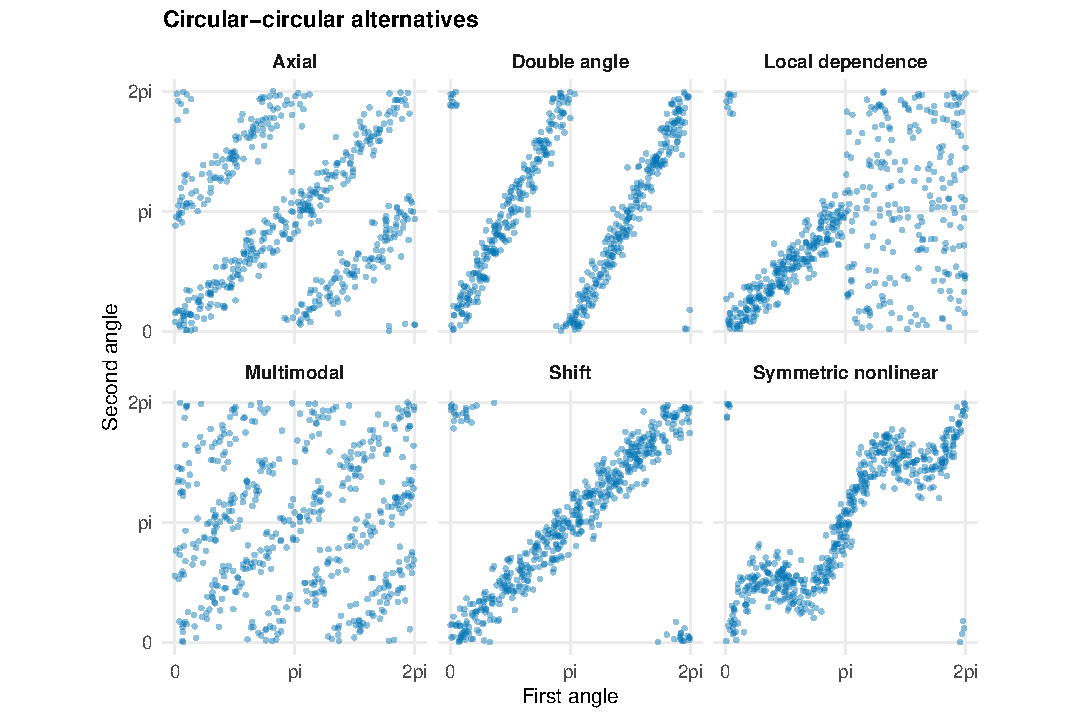
\includegraphics[width=.95\textwidth]{output/final/figures/fig1_alternatives.pdf}
\caption{Illustrative circular-circular alternatives used in the simulation study. Angles are shown in radians on \([0,2\pi)\).}
\label{fig:alternatives}
\end{figure}

The circular-circular simulation methods are HSIC fixed with \(\kappa=2\) for both margins, HSIC median, standardized multi-scale HSIC on \(G=\{0.5,1,2,4,8,16,32\}\), a first-order trigonometric moment diagnostic motivated by \citet{garciaportugues2024trigonometric}, and naive Euclidean-angle HSIC as an anti-example.  The trigonometric diagnostic implemented here is not the full test of \citet{garciaportugues2024trigonometric}.  Jammalamadaka-Sarma and Fisher-Lee diagnostics \citep{jammalamadaka2001topics,fisherlee1983circular} are implemented and reported for the Noshiro example, but they are not included in the main simulation figures and tables.  Comparisons are interpreted scenario by scenario because the procedures target different aspects of dependence.

Figure~\ref{fig:type1} and Table~\ref{tab:type1} summarize type-I error under the independent circular marginals.  Across all null scenarios and implemented methods, rejection rates range from \(0.028\) to \(0.072\), which is compatible with the nominal level at the reported Monte Carlo resolution.  Figure~\ref{fig:power} and Table~\ref{tab:selected-power} summarize circular-circular power across the simulated alternatives and effect sizes.  Shift, double-angle, local and symmetric nonlinear alternatives are detected at high rates by the HSIC methods.  The axial and multimodal alternatives are more sensitive to kernel scale.  At \(n=200\) and \(\rho=8\), the multi-scale procedure reaches rejection rate \(1.000\) for both axial and multimodal alternatives, while the median heuristic gives \(0.124\) and \(0.042\), respectively.  Figure~\ref{fig:strategy} and Table~\ref{tab:strategy} compare the kernel-parameter strategies.  Table~\ref{tab:strategy} is descriptive: the average rejection rate depends on the simulation design and should not be read as a uniform ranking.

\begin{figure}[!htbp]
\centering
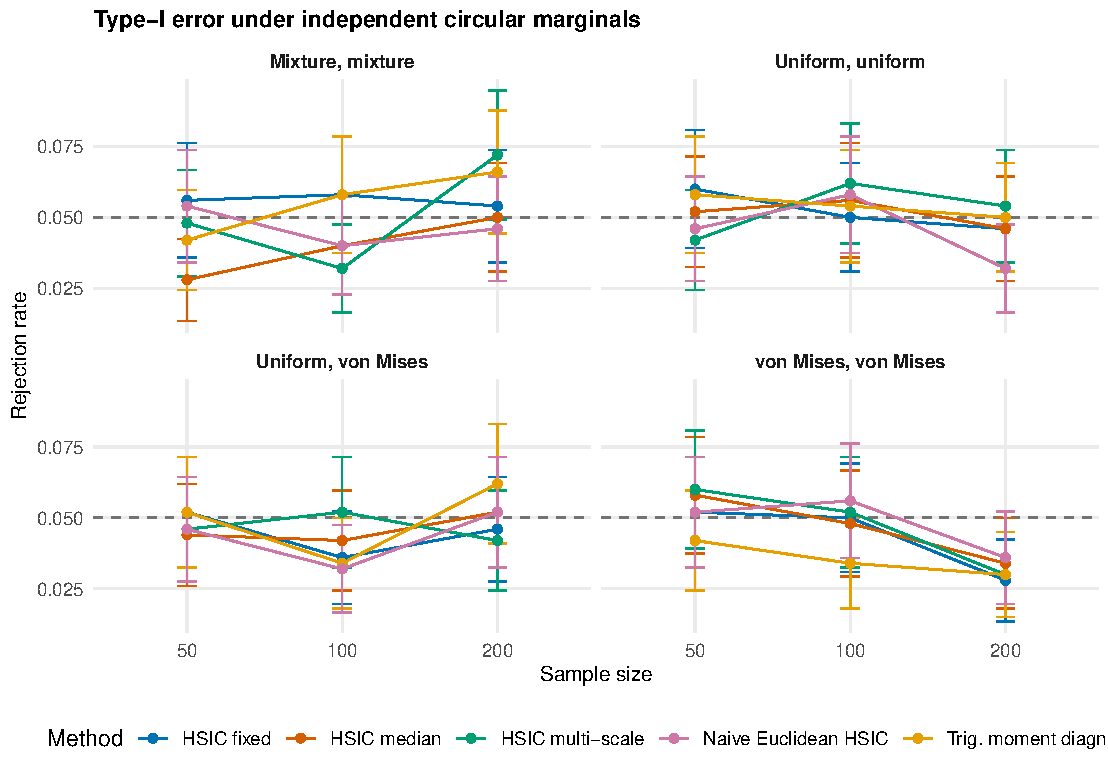
\includegraphics[width=.9\textwidth]{output/final/figures/fig2_type1.pdf}
\caption{Type-I error estimates under independent circular marginals. Error bars use Monte Carlo standard errors with \(R=500\), \(B=499\) and \(\alpha=0.05\).}
\label{fig:type1}
\end{figure}

\begin{table}[!htbp]
\centering
\scriptsize
\caption{Type-I error summary with Monte Carlo standard errors; alpha = 0.05.}
\label{tab:type1}
\begin{tabular}{llllllll}
\toprule
Scenario & n & Method & Reject. & MC SE & R & B & alpha
\\
\midrule
Mixture, mixture &  50 & HSIC fixed & 0.06 & 0.01 & 500 & 499 & 0.05\\
Mixture, mixture &  50 & HSIC median & 0.03 & 0.01 & 500 & 499 & 0.05\\
Mixture, mixture &  50 & HSIC multi-scale & 0.05 & 0.01 & 500 & 499 & 0.05\\
Mixture, mixture & 100 & HSIC fixed & 0.06 & 0.01 & 500 & 499 & 0.05\\
Mixture, mixture & 100 & HSIC median & 0.04 & 0.01 & 500 & 499 & 0.05\\
Mixture, mixture & 100 & HSIC multi-scale & 0.03 & 0.01 & 500 & 499 & 0.05\\
Mixture, mixture & 200 & HSIC fixed & 0.05 & 0.01 & 500 & 499 & 0.05\\
Mixture, mixture & 200 & HSIC median & 0.05 & 0.01 & 500 & 499 & 0.05\\
Mixture, mixture & 200 & HSIC multi-scale & 0.07 & 0.01 & 500 & 499 & 0.05\\
Uniform, uniform &  50 & HSIC fixed & 0.06 & 0.01 & 500 & 499 & 0.05\\
Uniform, uniform &  50 & HSIC median & 0.05 & 0.01 & 500 & 499 & 0.05\\
Uniform, uniform &  50 & HSIC multi-scale & 0.04 & 0.01 & 500 & 499 & 0.05\\
Uniform, uniform & 100 & HSIC fixed & 0.05 & 0.01 & 500 & 499 & 0.05\\
Uniform, uniform & 100 & HSIC median & 0.06 & 0.01 & 500 & 499 & 0.05\\
Uniform, uniform & 100 & HSIC multi-scale & 0.06 & 0.01 & 500 & 499 & 0.05\\
Uniform, uniform & 200 & HSIC fixed & 0.05 & 0.01 & 500 & 499 & 0.05\\
Uniform, uniform & 200 & HSIC median & 0.05 & 0.01 & 500 & 499 & 0.05\\
Uniform, uniform & 200 & HSIC multi-scale & 0.05 & 0.01 & 500 & 499 & 0.05\\
Uniform, von Mises &  50 & HSIC fixed & 0.05 & 0.01 & 500 & 499 & 0.05\\
Uniform, von Mises &  50 & HSIC median & 0.04 & 0.01 & 500 & 499 & 0.05\\
Uniform, von Mises &  50 & HSIC multi-scale & 0.05 & 0.01 & 500 & 499 & 0.05\\
Uniform, von Mises & 100 & HSIC fixed & 0.04 & 0.01 & 500 & 499 & 0.05\\
Uniform, von Mises & 100 & HSIC median & 0.04 & 0.01 & 500 & 499 & 0.05\\
Uniform, von Mises & 100 & HSIC multi-scale & 0.05 & 0.01 & 500 & 499 & 0.05\\
Uniform, von Mises & 200 & HSIC fixed & 0.05 & 0.01 & 500 & 499 & 0.05\\
Uniform, von Mises & 200 & HSIC median & 0.05 & 0.01 & 500 & 499 & 0.05\\
Uniform, von Mises & 200 & HSIC multi-scale & 0.04 & 0.01 & 500 & 499 & 0.05\\
von Mises, von Mises &  50 & HSIC fixed & 0.05 & 0.01 & 500 & 499 & 0.05\\
von Mises, von Mises &  50 & HSIC median & 0.06 & 0.01 & 500 & 499 & 0.05\\
von Mises, von Mises &  50 & HSIC multi-scale & 0.06 & 0.01 & 500 & 499 & 0.05\\
von Mises, von Mises & 100 & HSIC fixed & 0.05 & 0.01 & 500 & 499 & 0.05\\
von Mises, von Mises & 100 & HSIC median & 0.05 & 0.01 & 500 & 499 & 0.05\\
von Mises, von Mises & 100 & HSIC multi-scale & 0.05 & 0.01 & 500 & 499 & 0.05\\
von Mises, von Mises & 200 & HSIC fixed & 0.03 & 0.01 & 500 & 499 & 0.05\\
von Mises, von Mises & 200 & HSIC median & 0.03 & 0.01 & 500 & 499 & 0.05\\
von Mises, von Mises & 200 & HSIC multi-scale & 0.03 & 0.01 & 500 & 499 & 0.05\\
\bottomrule
\end{tabular}
\end{table}


\begin{figure}[!htbp]
\centering
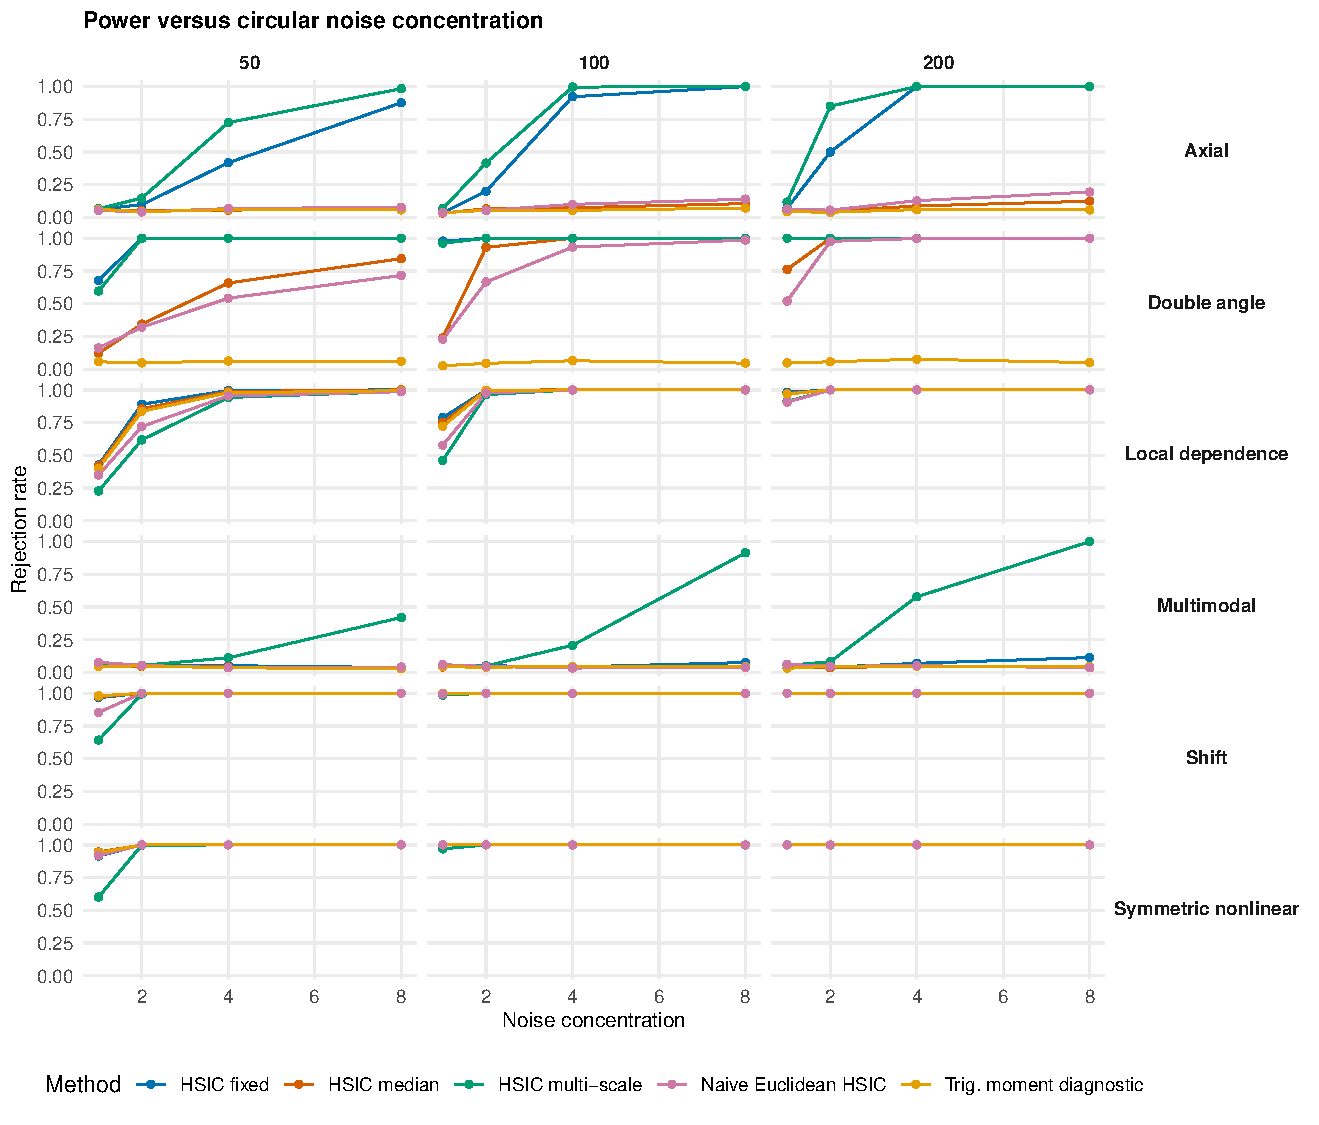
\includegraphics[width=.95\textwidth]{output/final/figures/fig3_power.pdf}
\caption{Circular-circular rejection rates by alternative and effect size. The simulation uses \(R=500\), \(B=499\) and \(\alpha=0.05\).}
\label{fig:power}
\end{figure}

\begin{table}[!htbp]
\centering
\scriptsize
\caption{Selected circular-circular rejection rates with Monte Carlo standard errors; alpha = 0.05.}
\label{tab:selected-power}
\begin{tabular}{lllllllll}
\toprule
Scenario & n & Method & Noise conc. & Reject. & MC SE & R & B & alpha
\\
\midrule
Axial & 200 & HSIC fixed & 8 & 1.00 & 0.00 & 500 & 499 & 0.05\\
Axial & 200 & HSIC median & 8 & 0.12 & 0.01 & 500 & 499 & 0.05\\
Axial & 200 & HSIC multi-scale & 8 & 1.00 & 0.00 & 500 & 499 & 0.05\\
Double angle & 200 & HSIC fixed & 8 & 1.00 & 0.00 & 500 & 499 & 0.05\\
Double angle & 200 & HSIC median & 8 & 1.00 & 0.00 & 500 & 499 & 0.05\\
Double angle & 200 & HSIC multi-scale & 8 & 1.00 & 0.00 & 500 & 499 & 0.05\\
Local dependence & 200 & HSIC fixed & 8 & 1.00 & 0.00 & 500 & 499 & 0.05\\
Local dependence & 200 & HSIC median & 8 & 1.00 & 0.00 & 500 & 499 & 0.05\\
Local dependence & 200 & HSIC multi-scale & 8 & 1.00 & 0.00 & 500 & 499 & 0.05\\
Multimodal & 200 & HSIC fixed & 8 & 0.11 & 0.01 & 500 & 499 & 0.05\\
Multimodal & 200 & HSIC median & 8 & 0.04 & 0.01 & 500 & 499 & 0.05\\
Multimodal & 200 & HSIC multi-scale & 8 & 1.00 & 0.00 & 500 & 499 & 0.05\\
Shift & 200 & HSIC fixed & 8 & 1.00 & 0.00 & 500 & 499 & 0.05\\
Shift & 200 & HSIC median & 8 & 1.00 & 0.00 & 500 & 499 & 0.05\\
Shift & 200 & HSIC multi-scale & 8 & 1.00 & 0.00 & 500 & 499 & 0.05\\
Symmetric nonlinear & 200 & HSIC fixed & 8 & 1.00 & 0.00 & 500 & 499 & 0.05\\
Symmetric nonlinear & 200 & HSIC median & 8 & 1.00 & 0.00 & 500 & 499 & 0.05\\
Symmetric nonlinear & 200 & HSIC multi-scale & 8 & 1.00 & 0.00 & 500 & 499 & 0.05\\
\bottomrule
\end{tabular}
\end{table}


\begin{figure}[!htbp]
\centering
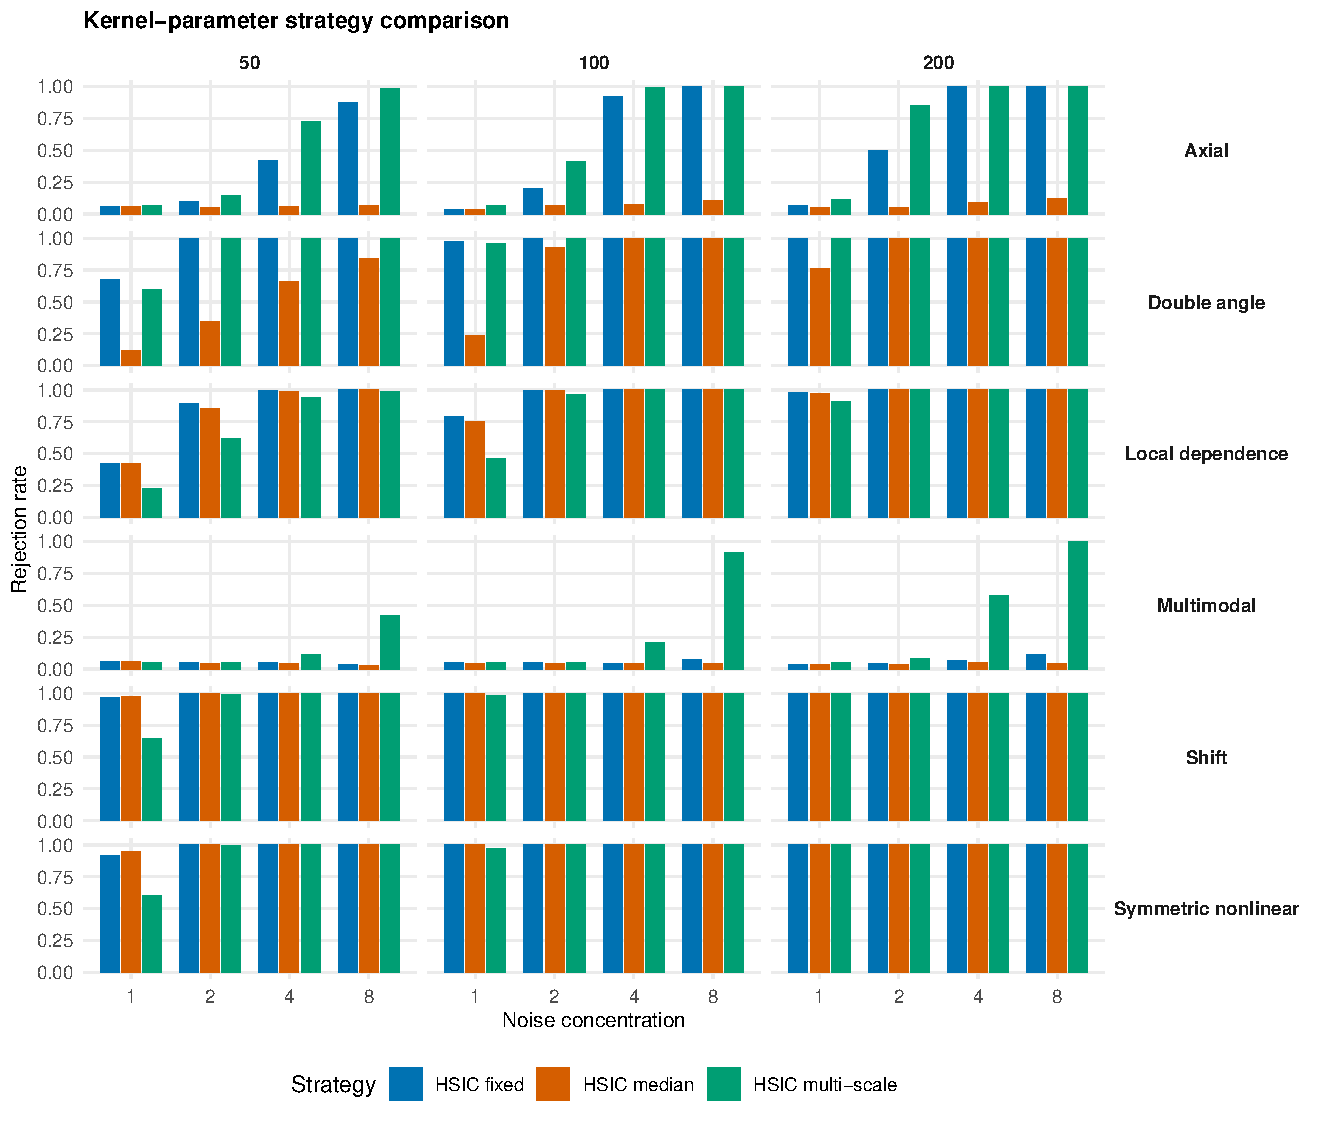
\includegraphics[width=.9\textwidth]{output/final/figures/fig4_strategy_comparison.pdf}
\caption{Comparison of fixed, median and standardized multi-scale HSIC strategies across the circular-circular alternatives. The simulation uses \(R=500\), \(B=499\) and \(\alpha=0.05\).}
\label{fig:strategy}
\end{figure}

\begin{table}[!htbp]
\centering
\scriptsize
\caption{Descriptive mean rejection rates for kernel-parameter strategies across the simulated circular-circular design; alpha = 0.05.}
\label{tab:strategy}
\begin{tabular}{llllll}
\toprule
Strategy & Mean reject. & Mean MC SE & R & B & alpha
\\
\midrule
HSIC fixed & 0.74 & 0.01 & 500 & 499 & 0.05\\
HSIC median & 0.63 & 0.01 & 500 & 499 & 0.05\\
HSIC multi-scale & 0.78 & 0.01 & 500 & 499 & 0.05\\
\bottomrule
\end{tabular}
\end{table}


\begin{figure}[!htbp]
\centering
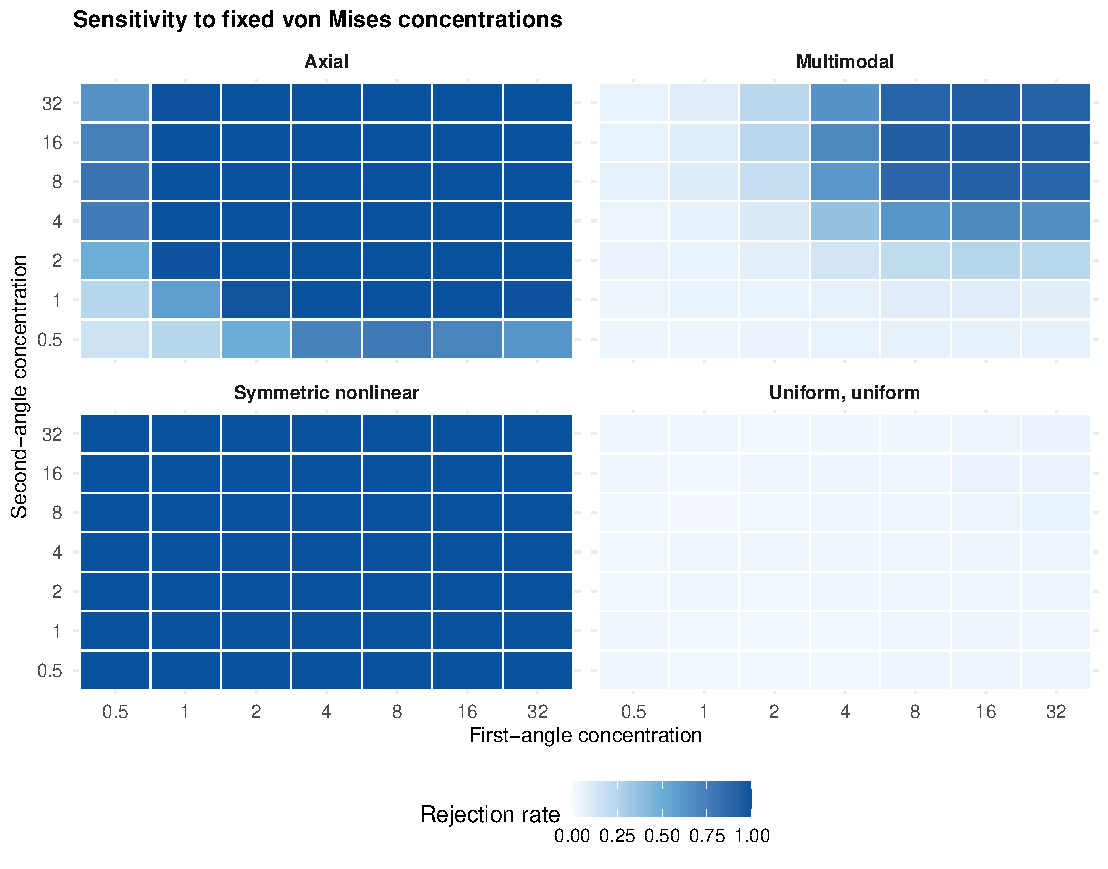
\includegraphics[width=.9\textwidth]{output/final/figures/fig5_kappa_sensitivity.pdf}
\caption{Reduced fixed-kernel sensitivity study for the independent null, axial, multimodal and symmetric nonlinear scenarios at \(n=100\). The alternative scenarios use \(\rho=8\), \(R=500\), \(B=499\) and \(\alpha=0.05\).}
\label{fig:kappa-sensitivity}
\end{figure}

For circular-linear simulations, \(\Theta\sim U(0,2\pi)\) and the Euclidean response is generated from four alternatives: \(X=1+\cos(\Theta-\pi/4)+\eta\), \(X=\cos(2\Theta)+\eta\), a four-dimensional trigonometric mean with coordinates \(\cos\Theta,\sin\Theta,\cos2\Theta,\sin2\Theta\), and a local mean shift on the arc \(\Theta\le\pi/2\).  The noise standard deviation is in \(\{0.3,0.5,0.7,1.0\}\).  The independent case uses a standard normal Euclidean response.  Figure~\ref{fig:cl-power} uses the single-scale circular-linear HSIC test with the median circular-distance rule for the von Mises concentration and the median Euclidean-distance rule for the Gaussian bandwidth; the Euclidean variables are used on their simulated scale without additional standardization.  The independent case remains close to nominal, with rejection rates between \(0.042\) and \(0.062\).  The first-harmonic and multivariate alternatives are detected strongly throughout this design, while the second-harmonic alternative weakens as linear noise increases.

\begin{figure}[!htbp]
\centering
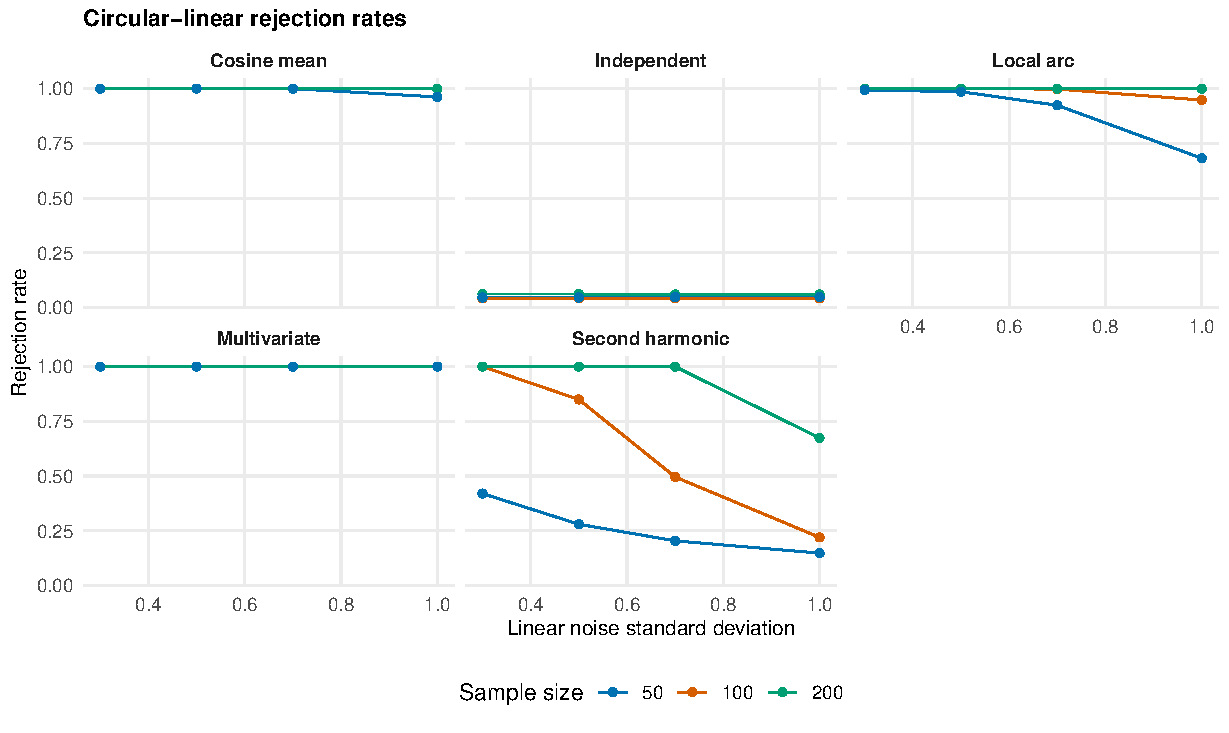
\includegraphics[width=.95\textwidth]{output/final/figures/fig6_circular_linear.pdf}
\caption{Circular-linear rejection rates for independent, harmonic, multivariate and local alternatives. The simulation uses \(R=500\), \(B=499\) and \(\alpha=0.05\).}
\label{fig:cl-power}
\end{figure}

Table~\ref{tab:torus-demo} gives a small torus-torus demonstration, included to check that the product-kernel implementation behaves as expected under the toroidal characteristic-kernel result in Proposition 1 and the subsequent toroidal-block HSIC consequence.  In this demonstration, \(X\in\mathbb T^2\) and \(Y\in\mathbb T^2\).  Under \(T0\), both toroidal variables have independent uniform coordinates.  Under \(T1\), the first coordinate of \(Y\) is \(X_1+\varepsilon\) modulo \(2\pi\), with \(\varepsilon\sim\mathrm{VM}(0,4)\), while the second coordinate of \(Y\) is independent uniform.  The torus product HSIC test uses concentration vector \((2,2)\) for both blocks, with \(n\in\{100,200\}\), \(R=250\), \(B=299\) and \(\alpha=0.05\).  This is not intended as an exhaustive toroidal power study.

\begin{table}[!htbp]
\centering
\scriptsize
\caption{Small torus-torus demonstration with Monte Carlo standard errors; alpha = 0.05.}
\label{tab:torus-demo}
\begin{tabular}{llllllll}
\toprule
Scenario & n & Method & Reject. & MC SE & R & B & alpha
\\
\midrule
T0\_independent & 100 & HSIC torus product & 0.07 & 0.02 & 250 & 299 & 0.05\\
T0\_independent & 200 & HSIC torus product & 0.06 & 0.01 & 250 & 299 & 0.05\\
T1\_coordinate\_coupled & 100 & HSIC torus product & 1.00 & 0.00 & 250 & 299 & 0.05\\
T1\_coordinate\_coupled & 200 & HSIC torus product & 1.00 & 0.00 & 250 & 299 & 0.05\\
\bottomrule
\end{tabular}
\end{table}


Table~\ref{tab:runtime} reports elapsed-time benchmarks for the three HSIC strategies.  These timings are machine dependent, but they illustrate the expected increase from single-scale to multi-scale testing.  The benchmark summary records Darwin 25.5.0 on arm64 with 14 logical cores available; the timing loop itself is sequential for each test call.

\begin{table}[!htbp]
\centering
\scriptsize
\caption{Runtime benchmark for HSIC strategies. Times are elapsed seconds with B = 199 permutations.}
\label{tab:runtime}
\begin{tabular}{lllllll}
\toprule
Method & n & B & Median sec. & IQR sec. & Reps & Cores
\\
\midrule
HSIC fixed &  50 & 199 & 0.007 & 0.003 & 20 & 14\\
HSIC fixed & 100 & 199 & 0.027 & 0.005 & 20 & 14\\
HSIC fixed & 200 & 199 & 0.102 & 0.020 & 20 & 14\\
HSIC median &  50 & 199 & 0.006 & 0.001 & 20 & 14\\
HSIC median & 100 & 199 & 0.027 & 0.007 & 20 & 14\\
HSIC median & 200 & 199 & 0.095 & 0.018 & 20 & 14\\
HSIC multi-scale &  50 & 199 & 0.306 & 0.041 & 20 & 14\\
HSIC multi-scale & 100 & 199 & 1.292 & 0.249 & 20 & 14\\
HSIC multi-scale & 200 & 199 & 4.335 & 0.855 & 20 & 14\\
\bottomrule
\end{tabular}
\end{table}


\FloatBarrier

\section{Real-data example: Noshiro directions}

The Noshiro example is retained as an applied demonstration, not as evidence of general superiority.  The data contain two angular variables: direction of steepest descent and direction of lateral ground movement.  The local data file is a CSV export of \texttt{ridgetorus::earthquakes} and records \(n=678\) observations with variables \texttt{theta1} and \texttt{theta2} in radians on \([0,2\pi)\), consistent with the \texttt{ridgetorus} documentation \citep{ridgetorusEarthquakes} and previous references \citep{hamada1992noshiro,rivest1997decentred,jones2015circulas}.  If the observations have spatial or sampling dependence, ordinary i.i.d. permutation p-values may be approximate.

Figure~\ref{fig:noshiro-torus} shows the binned torus representation of the Noshiro directions.  The fixed-grid Noshiro sensitivity calculation gives p-values equal to the minimum attainable value \(0.001\) at every retained grid point, so a nearly constant heatmap is not shown as a main figure.

Table~\ref{tab:noshiro} reports the Noshiro p-values using \(B=999\) permutations.  With add-one calibration, the smallest attainable p-value is \(1/(999+1)=0.001\).  These p-values should be read as evidence of association under the i.i.d. permutation model for this dataset, not as evidence that one method is generally superior.

\begin{figure}[!htbp]
\centering
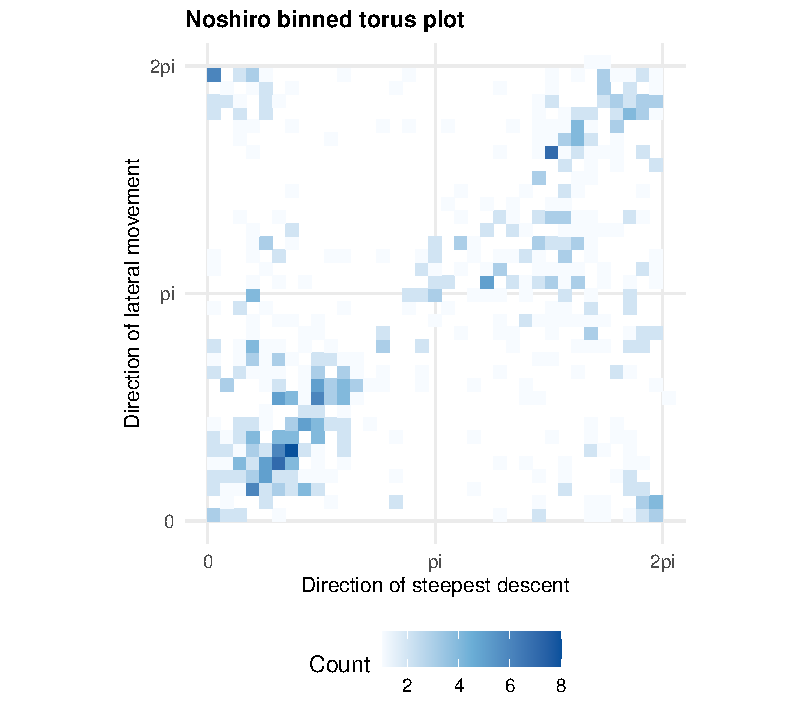
\includegraphics[width=.72\textwidth]{output/final/figures/fig7_noshiro_torus.pdf}
\caption{Binned torus plot for the Noshiro directional data. The first angle is direction of steepest descent and the second angle is direction of lateral movement, both in radians.}
\label{fig:noshiro-torus}
\end{figure}

\input{output/final/tables/table4_noshiro_p_values.tex}

\FloatBarrier

\section{Discussion}

The construction supports a focused message suitable for a computational statistics contribution: existing kernel independence ideas can be made directly usable for circular, toroidal and circular-linear data by choosing kernels that respect the geometry, proving the required characteristic property, and calibrating the empirical statistic by permutation.  The value is practical and statistical rather than foundational: the construction avoids raw-angle boundary artifacts, keeps the population HSIC interpretation in the circular and toroidal cases, and gives implementation-level guidance for kernel tuning.  The von Mises kernel provides a natural circle kernel because it is periodic, rotation invariant and characteristic.  Product kernels give a direct route to tori, and the circular-linear construction follows by pairing the circular kernel with a standard characteristic Euclidean kernel.

The standardized multi-scale test is a practical tuning device rather than a claim of uniformly optimal power.  It is useful because the search over concentration parameters is included in the permutation calibration, which avoids post hoc selection on the observed statistic.  Simulation comparisons with trigonometric moment diagnostics and naive Euclidean-angle HSIC, and the Noshiro diagnostics based on circular correlations, should therefore be interpreted scenario by scenario, since these procedures target different aspects of dependence.

Several limitations remain.  The computational cost is \(O(n^2B)\) for a single kernel pair and scales with the size of the multi-scale grid.  Ordinary permutations require exchangeability, so time series, trajectories and spatial data need resampling schemes that respect the sampling design.  Kernel choices affect finite-sample power, and a significant HSIC test does not by itself identify the mechanism or location of dependence.  The Noshiro analysis is consequently presented as an applied demonstration, not as evidence of general superiority.

Spherical and hyperspherical HSIC are natural extensions using von Mises--Fisher-type kernels, but they require a complete harmonic-analysis argument through spherical harmonics or Gegenbauer coefficients.  Distance covariance and RKHS-based dependence statistics are closely related in Euclidean and metric-space settings \citep{szekely2007distance,lyons2013metric,sejdinovic2013equivalence}; adapting that perspective to genuinely circular metrics is a separate direction rather than a comparator implemented here.  Further work includes conditional independence, local dependence maps, witness functions, block or spatial resampling schemes, and a maintained R package.

\section{Conclusion}

This paper presents a compact HSIC testing workflow for circular, toroidal and circular-linear data.  The central theoretical step is a Fourier proof that the von Mises kernel is characteristic on the circle, with product-kernel extensions to finite tori.  The empirical procedure combines the biased HSIC statistic, add-one permutation calibration and standardized multi-scale tuning.  The approach complements existing circular and directional independence tests by providing a geometry-aware kernel alternative with reproducible implementation.

\FloatBarrier

\section*{Code and data availability}

The R scripts and CSV files used to generate the reported analyses are included with the accompanying replication materials for this manuscript, available at \url{https://github.com/AurelienNicosiaULaval/geometry-aware-hsic-directional}.  The stable Zenodo concept DOI for the archived replication materials is \url{https://doi.org/10.5281/zenodo.20617102}.  The Noshiro data used here are stored as \texttt{data/noshiro.csv}, a local CSV export of the \texttt{earthquakes} data object from the \texttt{ridgetorus} R package; provenance notes are stored in \texttt{data/noshiro\_source.txt}.

\bibliographystyle{plainnat}
\bibliography{references}

\end{document}
